% Generated alongside scripts/make_figures.py.
\begin{figure}[t]\centering
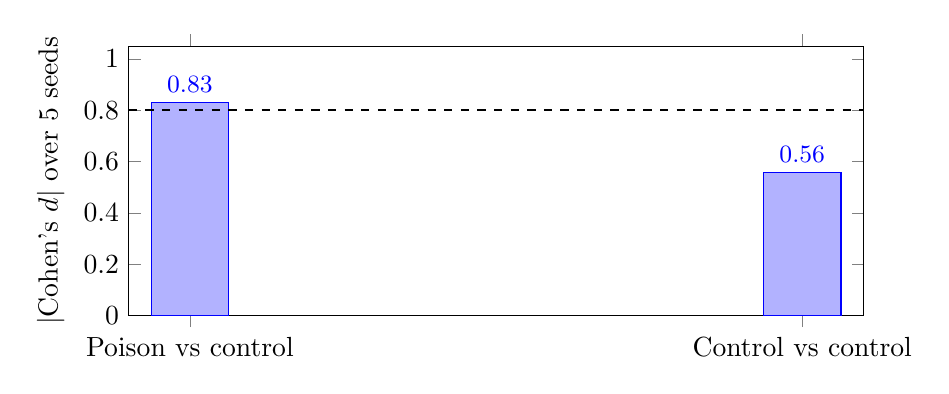
\begin{tikzpicture}
\begin{axis}[width=0.9\columnwidth,height=5cm,ybar,bar width=28pt,
  ytick={0,0.2,0.4,0.6,0.8,1.0},xtick={0,1},
  xticklabels={Poison vs control,Control vs control},
  ymin=0,ymax=1.05,ylabel={$|$Cohen's $d|$ over 5 seeds},
  nodes near coords,every node near coord/.append style={font=\small}]
\addplot coordinates {(0,0.831) (1,0.557)};
\draw[dashed,thick] ({rel axis cs:0,0}|-{axis cs:0,0.8}) -- ({rel axis cs:1,0}|-{axis cs:0,0.8});
\end{axis}
\end{tikzpicture}
\caption{The gating effect size beside its own negative control. The poison-vs-control measurement clears the pre-registered $d \geq 0.80$ bar (dashed), but the control-vs-control arm --- in which nothing is attacking anything --- reaches $|d| = 0.557$ on the same five seeds. A bar that a pure negative control can approach is not separating signal from noise at this sample size.}
\label{fig:floor}
\end{figure}
